\documentclass{article}


% if you need to pass options to natbib, use, e.g.:
%     \PassOptionsToPackage{numbers, compress}{natbib}
% before loading neurips_2021

% ready for submission
\PassOptionsToPackage{numbers, compress}{natbib}
\usepackage[preprint]{neurips_2021}
\bibliographystyle{abbrvnat}

\usepackage[utf8]{inputenc} % allow utf-8 input
\usepackage[T1]{fontenc}    % use 8-bit T1 fonts
\usepackage[colorlinks=true]{hyperref}       % hyperlinks
\usepackage{url}            % simple URL typesetting
\usepackage{booktabs}       % professional-quality tables
\usepackage{amsfonts}       % blackboard math symbols
\usepackage{nicefrac}       % compact symbols for 1/2, etc.
\usepackage{microtype}      % microtypography
\usepackage{xcolor}         % colors
\usepackage{siunitx}
\usepackage{graphicx}

\newcommand{\todo}[1]{{\color{red}todo: #1}}

\title{Spotify feat. Logistic Regression - \\ Popularity, Nothing Else Matters}

% The \author macro works with any number of authors. There are two commands
% used to separate the names and addresses of multiple authors: \And and \AND.
%
% Using \And between authors leaves it to LaTeX to determine where to break the
% lines. Using \AND forces a line break at that point. So, if LaTeX puts 3 of 4
% authors names on the first line, and the last on the second line, try using
% \AND instead of \And before the third author name.

\author{%
  Sebastian Hoffmann\thanks{correspondence to \texttt{sebastian.hoffmann@student.uni-tuebingen.de}}\\
  University of Tübingen\\
  Matriculation number 5954377\\
  \And
  Yannick Streicher\thanks{correspondence to \texttt{yannick.streicher@student.uni-tuebingen.de}}\\
  University of Tübingen\\
  Matriculation number 5331817\\
}

\begin{document}

\maketitle

\begin{abstract}
  What is the musical taste of the world? With the recent rise and global pervasiveness of music streaming services, such as Spotify, Deezer, or Apple Music, answering this question has become tractable. For this, we plan to analyze a \href{https://www.kaggle.com/rodolfofigueroa/spotify-12m-songs}{subset of 1.2 million songs} scraped from Spotify. However, this dataset lacks crucial information about popularity. Thus, an important step of our work is to augment the dataset further by querying the official Spotify REST API for a randomly sampled subset of the data. Besides a birds-eye overview of the musical landscape, e.g. distribution of genres, we want to identify common musical properties shared by popular songs, and likewise, very unpopular songs, using logistic regression. Such properties can be, for instance, tempo, mode, or key.
\end{abstract}

\section{Introduction}
%% general overview - i) we want dataset and clusters, ii) we want to predict popularity
The large amount of digital music today can be daunting. To successfully navigate this space, we urgently need better knowledge of the key characteristics of this opaque, highdimensional space. With our work, we want to present two important findings that contribute to this goal in a twofold manner: \textit{First} we create a clear overview of the musical landscape. That is, by applying t-SNE (\todo{cite?}) we show a twodimensional embedding of the high dimensional space of audio tracks. We find clusters that can be labeled as musical \textit{genres}. \textit{Second}, we zoom in and, using logistic regression, distill audio features that are of particular interest when considering the popularity of an audio track.

% motivation for the data: aggregate popularity measures with audio features
% or, we are guided by spots popularity measure
To predict the popularity of a song given its Spotify features, we have to find good labels that discriminate popular and unpopular songs.
To measure users responses to individual songs, Spotify presents two metrics, \textit{(i): Popularity:} An algorithmically determined integer between 0 and 100 (more is better), based on the total number of (recent) plays a track has. Artist popularity is derived from the popularity of its individual tracks. The second feature is \textit{(ii): Followers} which is the number of accounts that subscribed to this artists Spotify feed. The number can be interpreted as peoples interest in following the new releases of a particular artist.

\section{Dataset}

While Spotify provides data about individual songs or artists via its API, it does, however, not provide a catalogue of available songs on its platform. Thus, we use a dataset\footnote{\url{https://www.kaggle.com/rodolfofigueroa/spotify-12m-songs}} of $1.2$ million songs made available on Kaggle, a subset of the $70$ million songs accessible on Spotify~\cite{ingham_2020}. This dataset was created by first downloading the \href{https://musicbrainz.org/}{MusicBrainz} catalogue, an open-collaboration database of music releases, and then querying the Spotify API. 

For each song listed, the dataset contains basic meta informations such as artist and song name, as well as a set of $14$ song features that are provided by Spotify. These features include, among others, the estimated tempo, key, \emph{energy}, \emph{danceability}, or duration of the song. For a full list, refer to the Spotify API documentation. Crucially, the \emph{popularity} or genre of a song is not included in this dataset.

\subsection{Augmentation}
In a first step we retrieve additional information of all $85,113$ artists appearing in the dataset from the Spotify API. This information include the populartiy of that artist, aggregated from individual songs, the number of followers, and optionally a list of genres the artist is associated with.

Additionally, we query the Spotify API for every song in the dataset to obtain its individual popularity. While Spotify does not provide genre information at song level, we use the genre information associated with the first artist to further augment the dataset. The exact procedure is described in Section~\ref{sec:genre_clustering}. 

\subsection{Filtering}

\begin{figure}[t]
  \centering
  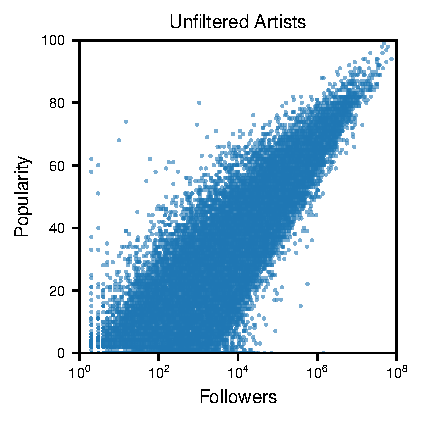
\includegraphics[width=0.38\textwidth]{../figures/artists_unfiltered.pdf}
  \qquad
  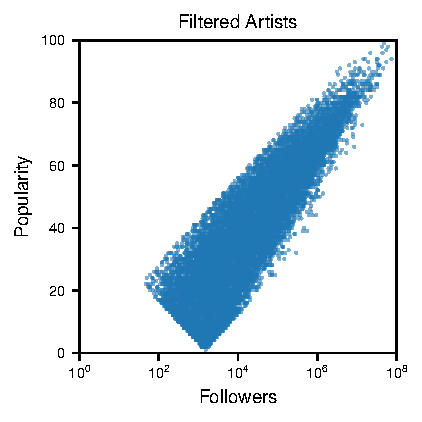
\includegraphics[width=0.38\textwidth]{../figures/artists_filtered.pdf}
  \caption{\textit{Left}: Artist popularity against log-followers before applying our filtering rules. \textit{Right}: We use the result of PCA to exclude artists that are outliers with respect to the first and second principal component.}
  \label{fig:filtering}
\end{figure}

To reduce potential noise introduced by unknown self-published artists, we want to restrict our analysis to those that can be considered professional or semi-professional musicians. This step was deemed necessary, as self-published artists do not undergo the feedback and quality control process a regular music label would provide. Indeed, we find that a quarter of artists on Spotify have less than $45$ followers and half of all artist have less than $393$. For comparison, \emph{Merikan}, a relatively unknown Drum and Bass producer, has $4581$ follower at the time of writing.

We find that the number of followers is roughly exponentially distributed. After applying a logarithmic transform, a clear linear relationship between the number of log-followers and popularity is visible (Pearson correlation coefficient: $0.88$, c.f. Fig.~\ref{fig:filtering},~left). 

Based on the popularity and log-follower count, we derive a robust filter criterion using principal component analysis~(PCA)~\cite{jolliffe2016principal}. After applying PCA, the first principal component is treated as a measure of the successfulness of an artist, taking both his popularity and followers into account. We threshold this measure to only include $50\%$ of all artists. Furthermore, we threshold the second component as well to remove outliers, i.e. artists with a high discrepancy between popularity and follower count. This step affects $1.6\%$ of all artists. Finally, we exclude those without associated genres.

In total, if all three steps are applied, $62.8\%$ of all artists are removed from the dataset and $31694$ artists in total are retained. This reduces the number of songs left in the dataset to $755472$ ($62.75\%$ of the original size).

\subsection{Finding metagenres by clustering}
\label{sec:genre_clustering}
The genres associated with an artist are often very fine-granulated. Out of \todo{$111$} genres in total, only \todo{$111$} have more than \todo{$123$} artists associated with them. To reduce the number of overall genres to a handful of overarching \emph{metagenres}, such as Rock, Jazz, or Hip-Hop, we employ agglomerative clustering~\cite{ward1963hierarchical} (we use~\cite{scikit-learn}). Agglomerative clustering lends itself naturally for this task as it exploits the inherent hierachical relationship between genres.

Inspired by constrastive methods~\cite{mikolov2013efficient, chen2020simple}, we exploit the fact that related genres are more likely to be associated with the same artist to construct a distance measure. In a first step, a similarity measure $s_{i, j} = (2 n_{ij}) / (N_i + N_j)$ between the $i$-th and $j$-th genre is defined, where $n_{ij}$ denotes the number of times they appear together and $N_i, N_j$ the total counts of the $i$-th and $j$-th genre respectively. The distance can then be defined as the reciprocal of that similarity measure. We then use this distance measure for the clustering procedure.

By running the clustering algorithm on an aggressively filtered subset of genres, we find $32$ metagenres, among them Jazz, Classical, Metal, Rock, Pop, or EDM, but also Soundtrack, or Show Tunes\footnote{Metagenres have been manually annotated}. These cover $60.5\%$ of all songs in the filtered dataset. To further improve coverage of songs, we rerun the clustering with less aggressive filtering to include more fine-grained genres. We then manually append these additional subgenres to the appropriate metagenre if applicable. This improves coverage to $71.3\%$.

\section{Experiments}

\subsection{Feature exploration}

Before 

\subsection{Logistic Regression}
% implicit assumtion: popularity = f(audio features)
For this project, the variable of interest is being \textit{popular} vs. \textit{unpopular} for individual tracks.
For the prediction we consider the \textit{audio features} for each of the tracks. 
Those features are purely technical and, therefore, we inductively assume that the probability whether a song is popular is only dependent on its audio features. 

% thresholding at 10%, 50% => inbalanced groups in 10% dataset
To create the labels, we apply a threshold to the popularity measure. 
We perform two different experiments. 
One with tight threshold, labeling only the top \SI{10}{\percent} songs as popular, and one more general one, where we use the median to divide the track into two groups.
As the tight threshold dataset contains a lot more unpopular songs than popular songs, the corresponding logistic regression model easily gets stuck in predicting \textit{unpopular} for all training examples. 
To address this issue, we follow the state of the art and use a \textit{weighted loss} function to penalize this behavior~\cite{haixiangLearningClassimbalancedData2017a}.

% training
We split the dataset into \SI{80}{\percent} training and \SI{20}{\percent} test data.
For both logistic regression models we apply l2-regularization and select the best hyperparameters via grid search, using 5-fold cross validation. 
Then, the final models are evaluated on individual test sets, respecting their popularity threshold.
Despite having a higher ROC-AUC score (tight model: \num{0.73} vs. wide model: \num{0.68}) the tight model performs worse at predicting the probability of being popular for individual songs, as seen in the calibration plots in Fig.~\ref{fig:logis_eval}, left.

% weight interpretation - elaborate what stood out
To find out how individual features influence the prediction we look into the learned coefficients of the better performing regression model, c.f.~Fig.\ref{fig:logis_eval}, right.
Weights in logistic regression have a linear relationship with the \textit{odds} of an outcome of the target variable.
Our analysis shows, that especially \textit{loudness} and \textit{danceability} correspond to higher odds of being popular.
These findings align with phenomena such as the \textit{loudness war}\cite{vickers2010loudness} of recorded music which emerged in the last years.
On the flip side, \emph{acousticness} and \emph{instrumentalness} negatively predict the odds, as well as \emph{valence} and \emph{energy}.


\begin{figure}
  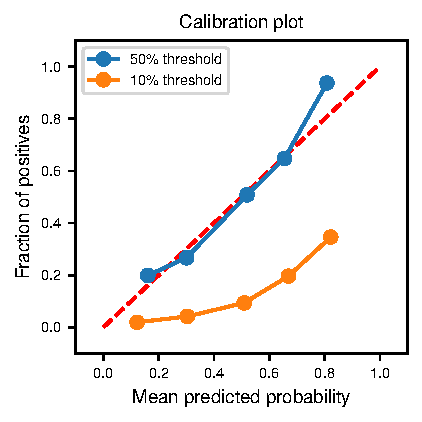
\includegraphics[width=0.42\textwidth]{../figures/calibration_combined.pdf}
  \qquad
  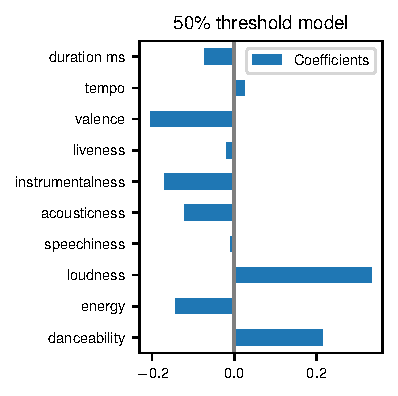
\includegraphics[width=0.42\textwidth]{../figures/logistic_coefs_50_threshold_model.pdf}
  \caption{\textit{Left}: Calibration plot following the methodology of \cite{niculescu-mizilPredictingGoodProbabilities2005}. The prediction space is discretized into 5 bins. Using the test set, for each bin, we plot the fraction of true popular songs against the mean predicted probability for those songs. \textit{Right}: The coefficients of the selected model for each audio feature. For the interpretation of individual features consider the API documentation of Spotify.}
  \label{fig:logis_eval}
\end{figure}

% \begin{figure}
%   \centering
%   \includegraphics[width=0.42\textwidth]{../figures/roc_logistic.pdf}
%   \caption{Parameters}
%   \label{fig:params}
% \end{figure}
  

\section{Discussion}

% does our dataset represent the population? Can we express certaintly?

% Logistic Discussion
%% limitations 1: Popularity Label Selection
In our experiments we binned songs by their popularity score into two classes. However, one could argue whether popularity is a discrete or a continuous quantity. Using logistic regression with multiple classes lead to worse results. That is, because the more popular classes are highly imbalanced in contrast to the unpopular classes, and weight-based approaches lead to general overestimation of popularity.
One would potentially have to investigate the under-the-hood workings of Spotify's popularity score to find a good representation of our interests.

%% Limitations 2: Popularity is not a function of Audio features
%% Loudness only shows that popular songs are high-end productions
Our logistic model revealed some features to potentially predict the popularity value of individual songs, but the results are to some extent dissonant. Because they express a somewhat similar emotion, one would expect \emph{energy, valence} and \emph{danceability} to influence the prediction in the same direction. Especially, since the latter two are correlated by \num{0.59}.
% Moreover, the pairwise correlation of the audio features is relatively high in this dataset which additionally unsharpens the interpretability of the model's parameters.
We distilled \emph{loudness} as the most influential audio feature. 
\emph{Does it mean, songs with higher loudness are more popular?} Modelling popularity as a function of audio features is brave. The results present us the evidence that there are important confounding factors that apply to song popularity. 
Popular artists have access to high-end audio production studios. This could be reflected in the loudness weight.
But, finally, finding that \textit{danceability} correlates with higher odds of being popular could potentially be an indication that gives hints to the answer of our overall thesis~-~humankind seems to like music that one can dance to.


\bibliography{bibliography}

\begin{appendix}
\section{Appendix}

\newpage

\begin{figure}
  \centering
  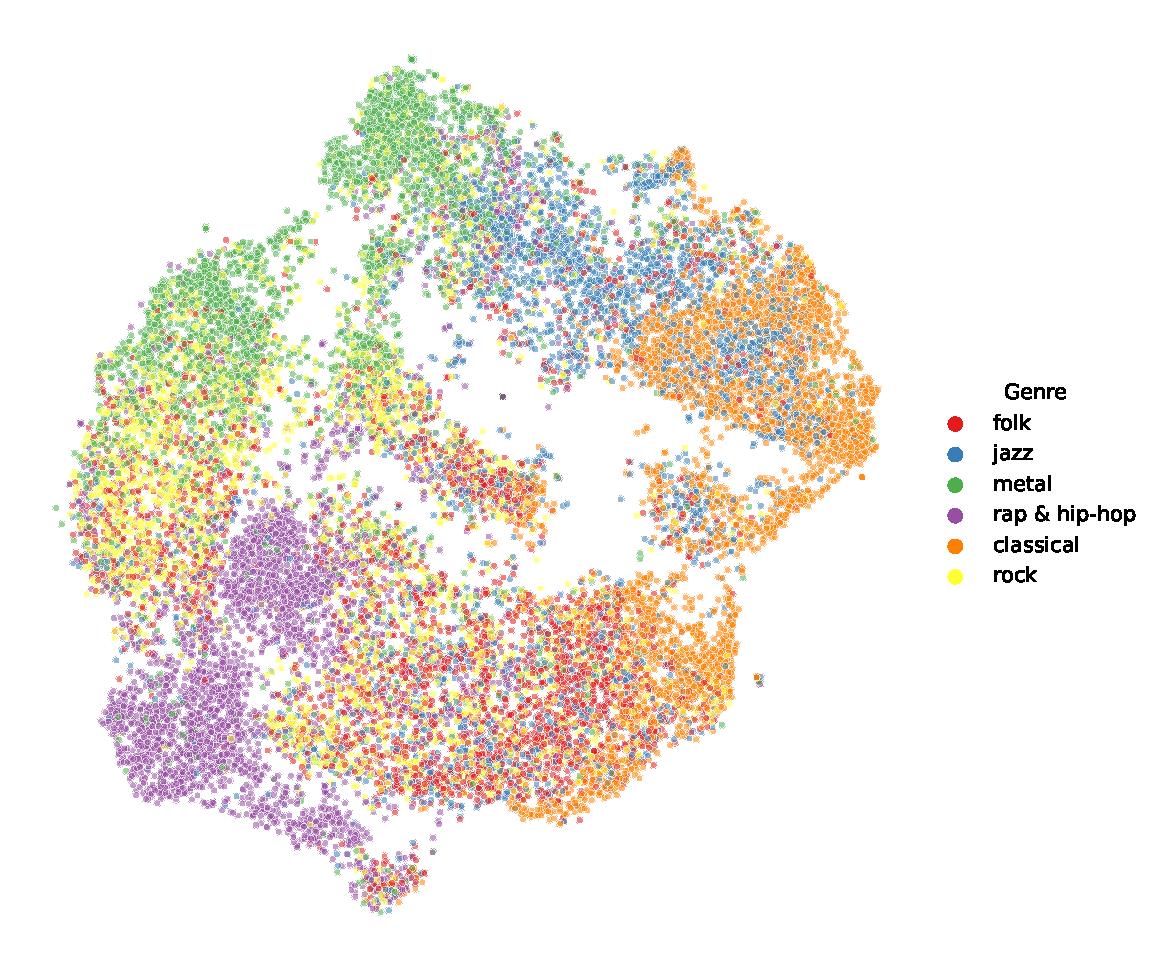
\includegraphics[width=1.0\textwidth]{../figures/tsne_genres.pdf}
  \caption{tsne}
  \label{fig:tsne_genres}
\end{figure}

\end{appendix}

\end{document}
